\documentclass[article]{jss}

\author{Fridolin Wild\\Wirtschaftsuniversit\"at Wien \And
David Meyer\\Wirtschaftsuniversit\"at Wien}

\title{\pkg{lsa}: an \proglang{R} Package for Latent Semantic Analysis}

\Plainauthor{Fridolin Wild, David Meyer} 
\Plaintitle{lsa: an R Package for Latent Semantic Analysis}
\Shorttitle{Latent Semantic Analysis}

\Abstract{
  Latent semantic analysis (LSA) has continuously stirred scientific interest
  since its invention in the early 1990ies. LSA combines the classical 
  vector space model -- well known in textmining -- with a 
  singular value decomposition (SVD), a two-mode factor analysis. Thereby, 
  bag-of-words representations of texts can be mapped into a modified 
  (=higher-order) vector space that is assumed to reflect semantic 
  structure. 
  
  LSA can be applied for various purposes, e.g. to automatically evaluate 
  free text responses typical for educational assessments, to find relevant documents
  matching unstructured queries typical in an information retrieval setting,
  or to detect homologies between protein sequences as applied in bioinformatics. 
  % or to detect new classification schemes.
 
  In this paper a description of the \pkg{lsa} package for the language and
  environment \proglang{R} is given and its proper use is illustrated through 
  examples from a set of different application domains. Besides the high-level
  core functionalities implementing the LSA process, the package includes
  several sets of supporting functions facilitating the LSA process in the 
  construction of the input matrices, the application of preprocessing 
  methods and weighting schemes, the selection of the desired 
  number of factors, and the calculation of similarities within a 
  latent-semantic space.

}

\Keywords{lsa, latent semantic analysis, text technology, computer linguistics, \proglang{R}}
\Plainkeywords{lsa, latent semantic analysis, text technology, computer linguistics, R}

%% publication information
%% \Volume{13}
%% \Issue{9}
%% \Month{September}
%% \Year{2004}
%% \Submitdate{2004-09-29}
%% \Acceptdate{2004-09-29}

\Address{
  Fridolin Wild, David Meyer\\
  Institute for Information Systems and New Media\\
  Vienna University of Economics and Business Administration\\
  A-1090 Vienna, Austria\\
  E-mail: \email{firstname.surname@wu-wien.ac.at}
}

\begin{document}
\setcounter{equation}{0}
\renewcommand{\thefigure}{\arabic{figure}}
\renewcommand{\theequation}{\arabic{equation}}

\section[introduction]{Introduction}

Semantics, -- the study of meaning --, is usually defined to investigate 
the relation of signs to their corresponding objects. These representations
of objects and (among others) their relations, interactions, properties,
and states can be generated in various ways, e.g. consciously as well as
unconciously by the human brain, intellectually explicated and formalised
in a manifold of different representation formats, or automatically derived 
from data by machines.

One branch of automated techniques (`heuristics-based approaches') 
in generating representations consists of algorithms that take utterances 
specified in a particular language with a certain grammar and try 
to data mine their semantic structure from collocation heuristics.

Latent Semantic Analysis (LSA\footnote{Often also named Latent Semantic
Indexing (LSI).}), is one of these methods. Originally, LSA was introduced 
to facilitate the investigation of meaning in texts. By now, LSA,
however, has been applied in several different domains, also 
dealing with non-natural language data specified in structured form or
in even in formal languages (see Section X below). In this paper we
therefore use the term `text' to denote a compilation of language utterances 
regardless of their complexity level, we do not want to differentiate 
between e.g. German prose, RDF triples, or genome sequences. As the core LSA 
process is position insensitive, these texts are generally treated as bags of words.

The basic idea behind LSA is that texts have a semantic structure, which, 
however, is obscured by word usage (e.g. through synonymy or polynomy). 
It is assumed, that by using conceptual indices derived statistically from 
coocurrences via a truncated singulare value decomposition this latent-semantic 
structure can be unveiled, cf. \cite{landauer:1990}.

LSA is a representation theory (cf. \cite{kintsch:1998}) in the sense, that it 
specifies a representation process about how to generate a representation 
product (cf. \cite{scaife:1996}). However, as Perfetti (\cite{perfetti:1998}) 
points out in general for all cooccurrence based systems, it is not yet a fully
matured representation theory, especially when applied exclusively over 
cooccurrences.

LSA has been applied in various application areas. Deerwester et al. 
used LSA for indexing and information retrieval, finding a significant increase 
in precision and recall compared to e.g. simple term matching (\cite{landauer:1990}). 
Foltz used LSA for information filtering tasks 
in order to match incoming new documents against users' long-term interests 
specified in a profile (\cite{foltz:1990}). The Bellcore Advisor matches people 
instead of documents: user queries are compared with existing documents 
written by the experts available (\cite{furnas:1988}). Wu et al. used LSA
to classify protein sequences (\cite{wu:1995}). Dong et al. applied LSA in order to
remotely detect homologies between protein sequences (\cite{dong:2006}).

  
\section[method]{The Method}


\subsection{The Basic LSA Process}

In a typical LSA process, first a document-term matrix is constructed 
from a given text base of \begin{math}n\end{math} documents containing 
\begin{math}m\end{math} terms (see \begin{math}M\end{math} in figure~\ref{fig:process}). 
This matrix \begin{math}M\end{math} of the size \begin{math}m \times n\end{math} 
is then resolved by the singular value decomposition into the term vector 
matrix \begin{math}T\end{math} (constituting the right singular vectors), 
the document vector matrix \begin{math}D\end{math} (constituting the right 
singular vectors) being both orthonormal and the diagonal matrix 
\begin{math}S\end{math}, see Equation (1). 

\begin{equation}M = TSD^T\end{equation}

These matrices are then reduced to a particular number of 
dimensions \begin{math}k\end{math}, giving the truncated matrices \begin{math}T_{k}\end{math}, 
\begin{math}S_{k}\end{math} and \begin{math}D_{k}\end{math} --- the latent semantic space. 

Multiplying the truncated matrices \begin{math}T_{k}\end{math}, 
\begin{math}S_{k}\end{math} and \begin{math}D_{k}\end{math} as in Equation (2) 
results in a new matrix \begin{math}M_{k}\end{math} which is the least-squares best 
fit approximation of \begin{math}M\end{math} with \begin{math}k\end{math} 
singular values. \begin{math}M_{k}\end{math} is of the same format as 
\begin{math}M\end{math}, i.e., rows are the same terms, columns represent
the same documents.

\begin{equation}M_k = \sum\limits_{i=1}^k t_i \cdot s_i \cdot d_i^T\end{equation}

\begin{figure}\label{fig:process}
  \centering
  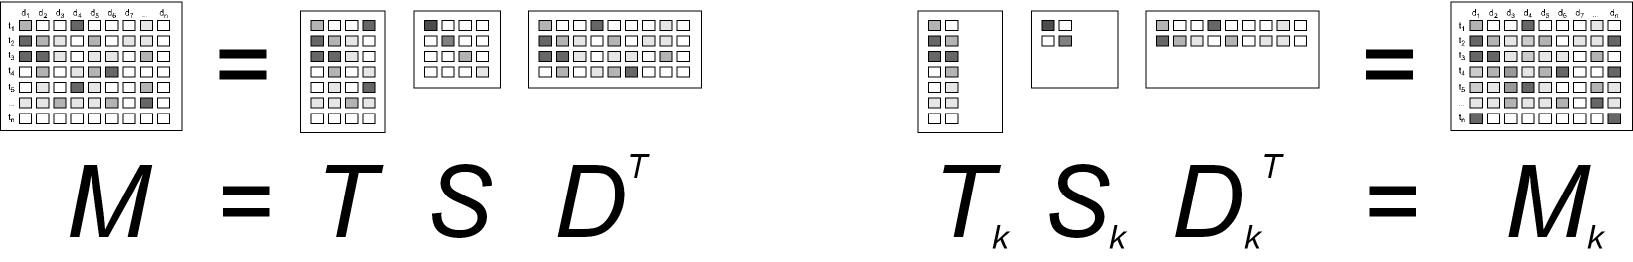
\includegraphics[width=140mm]{lsa_process.jpg}
  \caption{Singular Value Decomposition (original left, truncated right).}
\end{figure}

In the case of folding-in, i.e., multiplying new documents into a given
latent semantic space, the matrices \begin{math}T_k\end{math} and \begin{math}S_k\end{math} 
remain unchanged and an additional \begin{math}D_k\end{math} is created (without replacing the old one).
All three are multiplied together to return a (new and appendable)
document-term matrix \begin{math}\hat{M}\end{math} in the term-order 
of \begin{math}M\end{math}.

\subsection{Updating by Folding-In}

To keep additional documents from influencing the factor distribution
calculated previously from a particular text basis, they can be folded-in 
after the singular value decomposition. Therefore, the add-on documents can be 
added to the pre-exisiting latent semantic space by mapping them into the 
existing factor structure. Moreover, folding-in
is computationally a lot less costly, as no singular value decomposition
is needed.

Explicitly, a pseudo document vector \begin{math}\hat{m}\end{math} of the new documents 
is calculated into as shown in the equations (1) and (2) (cf. \cite{berry:1995}):

\begin{equation}\hat{d} = v^{T} T_{k} S_{k}^{-1}\end{equation}

The document vector \begin{math}v^T\end{math} in equation~(1) is identical to an additional 
column of an input textmatrix \begin{math}M\end{math} with the term frequencies of the 
document to be folded-in. \begin{math}T_k\end{math} and \begin{math}S_k\end{math} are the truncated matrices 
from the SVD on a given text collection to construct the latent semantic space. 

\begin{equation}\hat{m} = T_{k} S_{k} \hat{d}\end{equation}

The resulting vector
\begin{math}\hat{m}\end{math} from equation~(2) is identical to an additional column in the
textmatrix representation of the latent semantic space.

\subsection{Additional Steps of the Process}

Several steps can be functionally differentiated in
the whole latent semantic analysis process. Every step
introduces new parameters that drive the effectiveness
of the algorithm. The steps consist of textbase selection,
pre-processing of input texts, application of weighting-schemes, 
choice of dimensionality, and similarity measurement technique (see 
Figure~\ref{fig:steps}).

\begin{figure}\label{fig:steps}
  \centering
  \includegraphics[width=140mm]{lsa_steps_3.png}
  \caption{Typical steps in an LSA process.}
\end{figure}

Document pre-processing is a common procedure in information retrieval and 
comprises several text operations such as lexical analysis, use of stop-word 
lists, stemming, selection of index terms, and construction of thesauri (cf. \cite{baezayates:1999}).
 
Two stop-word list are provided with the package, a German one (containing 373 terms)
and an English one (containing ??? terms). As stemmer Porter's Snowball stemmer from
the package Rstem is deployed. Although research shows that document pre-processing 
in general yields better results in information retrieval this is not necessarily 
true for other application settings.

Weighting-schemes have shown to have the extensive influence on the effectiveness 
of LSA. Several weighting-schemes -- both local and global -- are provided. Two local 
term weighting schemes (logarithmised term frequency and binary term frequency) and 
three global (normalization, inverse document frequency, and entropy) are included.

Among other factors the choice of dimensionality has a significant impact on the 
results of any distance measurement conducted on the vector space of the 
underlying data. After the application of the singular value decomposition on 
the original term-document matrix, a reduced matrix it is reconstructed using only 
the k-largest singular values. This aims at an approximation to the original vector 
space by a reduction of the dimensionality. This approach captures the most important 
structure inherent in the original matrix, reducing noise and variability in 
word usage.

The way how and algorithm with which similarities are measured is another
influencing factor.

\section{Overview over the Package}

System Architecture Diagramme

\section{Illustrative Example (Landauer)}

landauer example?

\subsection{Data Model}

textmatrices, lsa spaces, triples, file in, (output)

\section{Building the Model: Constructing Latent Semantic Spaces}

abstract high level core methods

With \code{lsa()} a new latent semantic space can
be constructed over a given document-term matrix. To ease
comparisons of terms and documents with common
correlation measures, the space can be converted into
a textmatrix of the same format as \code{y} 
by calling \code{as.textmatrix()}.

the latent semantic space idea

fold-in

To add more documents or queries to this latent semantic
space in order to keep them from influencing the original 
factor distribution (i.e., the latent semantic structure calculated
from a primary text corpus), they can be `folded-in' later on 
(with the function \code{fold\_in()}).

Overview over influencing parameters for every core function.

\begin{table}
\centering
\caption{Weighting Schemes (tf = term frequency)}
\label{tab:schemes}
\begin{tabular}{p{30mm}@{\extracolsep{5mm}}p{80mm}}
\hline\noalign{\smallskip}
Call & Description \\
\noalign{\smallskip}\hline\noalign{\smallskip}
lw\_logtf() & $log(m_{i,j}+1)$ is applied on every cell \\
lw\_bintf() & $tf_{ij} = 1$, iff $tf_{ij} \neq 0$ \\
lw\_tf() & completely unmodified (placebo function) \\
gw\_idf() & $\log_2{\frac{ndocs}{df_i}+1}$, where $df_i = \sum\limits^j_1{\frac{tf_ij}{tf_ij}}$ \\
gw\_normalisation() & $\frac{1}{\sqrt{\sum\limits_{1}^{j}{tf^2_{ij}}}}$ \\
gw\_gfidf() & Global Frequency $\times$ idf: $\sum\limits_1^j{tf_{ij}} \times idf$ \\
entropy() & $-\sum\limits^{1}_{j}{\frac{p_{ij}\log{p_{ij}}}{\log{numdocs}}}$, where $p_{ij}=\frac{tf_{ij}}{\sum_j^1{tf_{ij}}}$ \\
gw\_entropy() & 1 + Entropy \\
\noalign{\smallskip}\hline
\end{tabular}
\end{table}


\section{Tuning the Model}

Choosing Hyperparameters, Influencing Parameters
term weightings: table with formulas

\section{Working with Latent Semantic Spaces}

comparing terms to terms,
comparing documents,
...

Correlation Measures

Visualisation

\subsection[example information retrieval]{Example 1: Matching Arabic Documents}


\subsection[example essay scoring]{Example 2: Automated Essay Scoring}

\begin{figure}\label{fig:essayscoring}
  \centering
  \includegraphics[width=100mm]{essay-scoring-overview.png}
  \caption{Basic work flow for essay scoring with LSA.}
\end{figure}


\subsection[example classification]{Example 3: Functional Relationships of Proteins}




\section[conclusions]{Conclusions}

Future plans.

\section[acknowledgements]{Acknowledgements}

Christina Stahl, Gerald Stermsek, Gustaf Neumann, Yoseba Penya, Kurt Hornik, Stefan Sobernig.
Art Graeser, Max Louwerse, Roberto Turrin, Brian Ripley, Milos Kravcik, Goto...

\bibliography{lsa}

\end{document}
